\documentclass[nonacm, sigplan,10pt]{acmart}

\settopmatter{printacmref=false} % remove ACM reference block
\renewcommand\footnotetextcopyrightpermission[1]{} % remove copyright footnote
\pagestyle{plain} % page numbers for class submission

\usepackage{amsmath}
\usepackage{microtype}
\usepackage{appendix}

\title{InsightProt: Latent Identity Inference from \\Protein Conformational Ensembles}

\author{Anna Su}
\affiliation{%
  \institution{Yale University}
  \city{New Haven}
  \state{CT}
  \country{USA}
}
\email{anna.su@yale.edu}

\begin{abstract}
Proteins are better modeled as distributions over conformational states than as single static structures.
This motivates a probabilistic treatment of \emph{molecular identity} as a latent variable inferred from multiple, heterogeneous structural observations.
This hypothesis is evaluated using multiscale Gauss Linking Integral (mGLI) embeddings and a variational latent-variable model on a subset of the ProteinConformers benchmark.
Preliminary results show that a learned latent representation assigns higher \emph{within-set coherence} to conformational ensembles arising from a single underlying protein than to mixed-protein ensembles, under a coarse structural observation operator.
\end{abstract}

\keywords{protein conformational ensembles, latent variable models, variational autoencoders, topological embeddings, Gauss linking integral}

\begin{document}
\maketitle

\section{Context}
Structural biology and molecular simulation routinely generate \emph{ensembles} of conformations for a given protein, reflecting energetic basins and functionally relevant state transitions.
Consequently, a protein is naturally associated with a distribution over structures.
Large-scale benchmarks such as \emph{ProteinConformers} provide physically realistic conformational ensembles at scale, enabling systematic study of representation learning across high-variance structural distributions \cite{ProteinConformers2025}.
In practice, structure comparison still relies heavily on deterministic geometric alignment (e.g., RMSD, TM-score) and residue-indexed features (e.g., contact maps) \cite{ZhangSkolnick2004TMscore}.
These methods are effective when residue correspondence and near-isometric deformation assumptions hold, but they do not explicitly model \emph{identity} as a latent factor underlying a multi-modal set of conformations.
This motivates studying representations that are stable under such deformations and support probabilistic inference from multiple observations.

\section{Introduction}
Let $z_{\mathrm{id}}$ denote a latent molecular identity and $z_{\mathrm{state}}$ a latent conformational state.
We adopt the generative view
\begin{equation}
x \sim p(x \mid z_{\mathrm{id}}, z_{\mathrm{state}}), \qquad
y = g(x),
\end{equation}
where $x$ is a high-resolution protein structure (e.g., atomic coordinates) and $y$ is an \emph{observation} obtained by an operator $g(\cdot)$ (e.g., coarse-graining, partial visibility, or featurization).
Given a set of observations $\{y_i\}_{i=1}^K$, the inference question is \emph{distributional consistency}:
do these observations plausibly arise from a single latent identity $z_{\mathrm{id}}$ across multiple states, or from multiple identities?
This is a model-selection problem in which evidence provides a natural criterion.

We hypothesize that topology-aware embeddings may better support this inference than purely local geometric signatures in regimes with large conformational variability.
In particular, the multiscale Gauss Linking Integral (mGLI) provides a deformation-stable, global descriptor of chain organization across spatial scales \cite{Shen2024mGLI}.
Unlike contact maps that depend on distance thresholds and residue indexing, mGLI integrates nonlocal geometric relationships and is invariant to rigid-body motions, suggesting improved stability under large continuous deformations.
Our goal is not to replace sequence-based identity checks when available, but to test whether, under coarse structural observations, identity is more naturally captured as a latent variable inferred probabilistically from ensembles.

\section{Methods and Preliminary Results}
From an initial pool of proteins with large conformational diversity, we select $N=50$ proteins and sample $K=10$ conformers per protein using a farthest-point heuristic based on structural dissimilarity, encouraging multimodal ensembles. An example protein and some of its conformers are visualized in PyMol \cite{pymol}(Fig.\ref{fig:conformers}).

\begin{figure}[h]
    \centering
    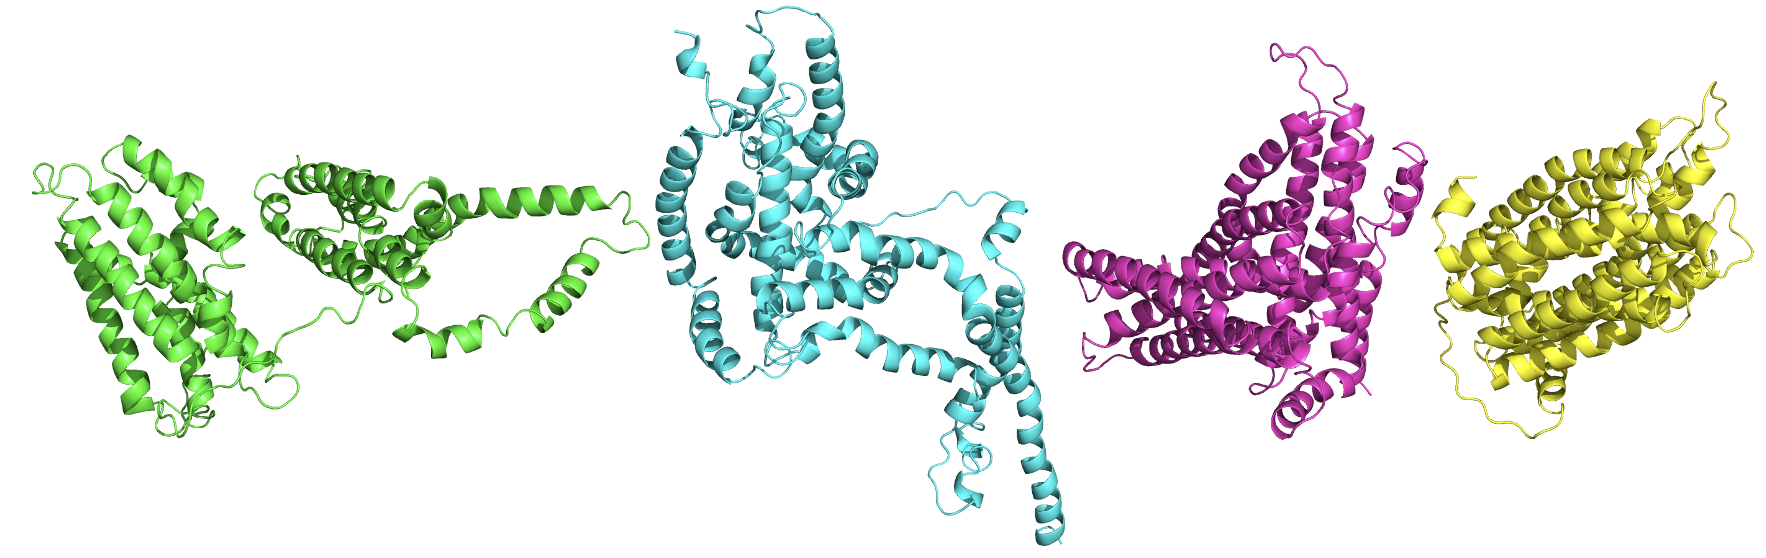
\includegraphics[width=0.9\linewidth]{Figures/conformers.png}
    \caption{Four conformers of an example protein showing high structural dissimilarity.}
    \label{fig:conformers}
\end{figure}

To avoid reliance on residue-level correspondence, we define a coarse observation operator $g(\cdot)$ that retains only backbone (C$_\alpha$) geometry.
Each observed structure is mapped to a fixed-length multiscale Gauss Linking Integral (mGLI) embedding~\cite{Shen2024mGLI}, yielding a global, deformation-stable descriptor.
A PCA projection of raw mGLI embeddings (Fig.~\ref{fig:pca_raw}) shows substantial overlap between proteins, indicating that identity is not linearly separable in the original feature space. PCA of protein centroids further confirms this (Fig. ~\ref{fig:pca_centroids}). 

\begin{figure}[h]
    \centering
    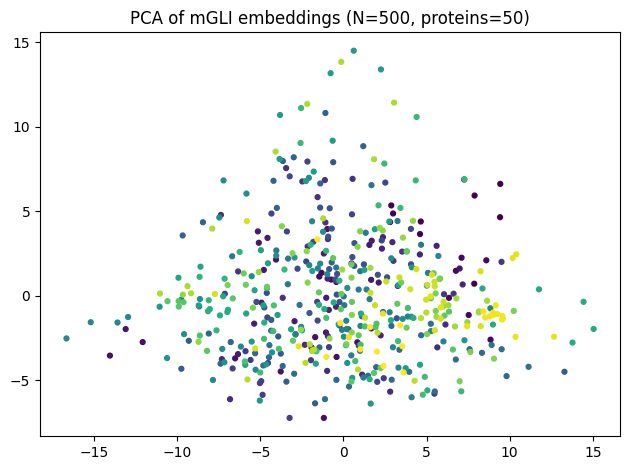
\includegraphics[width=0.9\linewidth]{Figures/raw_PCA.png}
    \caption{PCA of raw mGLI embeddings for $N=50$ proteins.}
    \label{fig:pca_raw}
\end{figure}

\subsection{Latent representation learning}
We train a variational autoencoder (VAE) on mGLI embeddings.
Near-constant embedding dimensions are removed prior to normalization to stabilize training.
The VAE is trained without identity labels, using early stopping based on validation loss (Fig.~\ref{fig:loss_curve}).
While training loss continues to decrease with additional epochs, validation loss plateaus after $\sim$300 epochs, motivating early stopping to preserve latent generalization.

\begin{figure}[h]
    \centering
    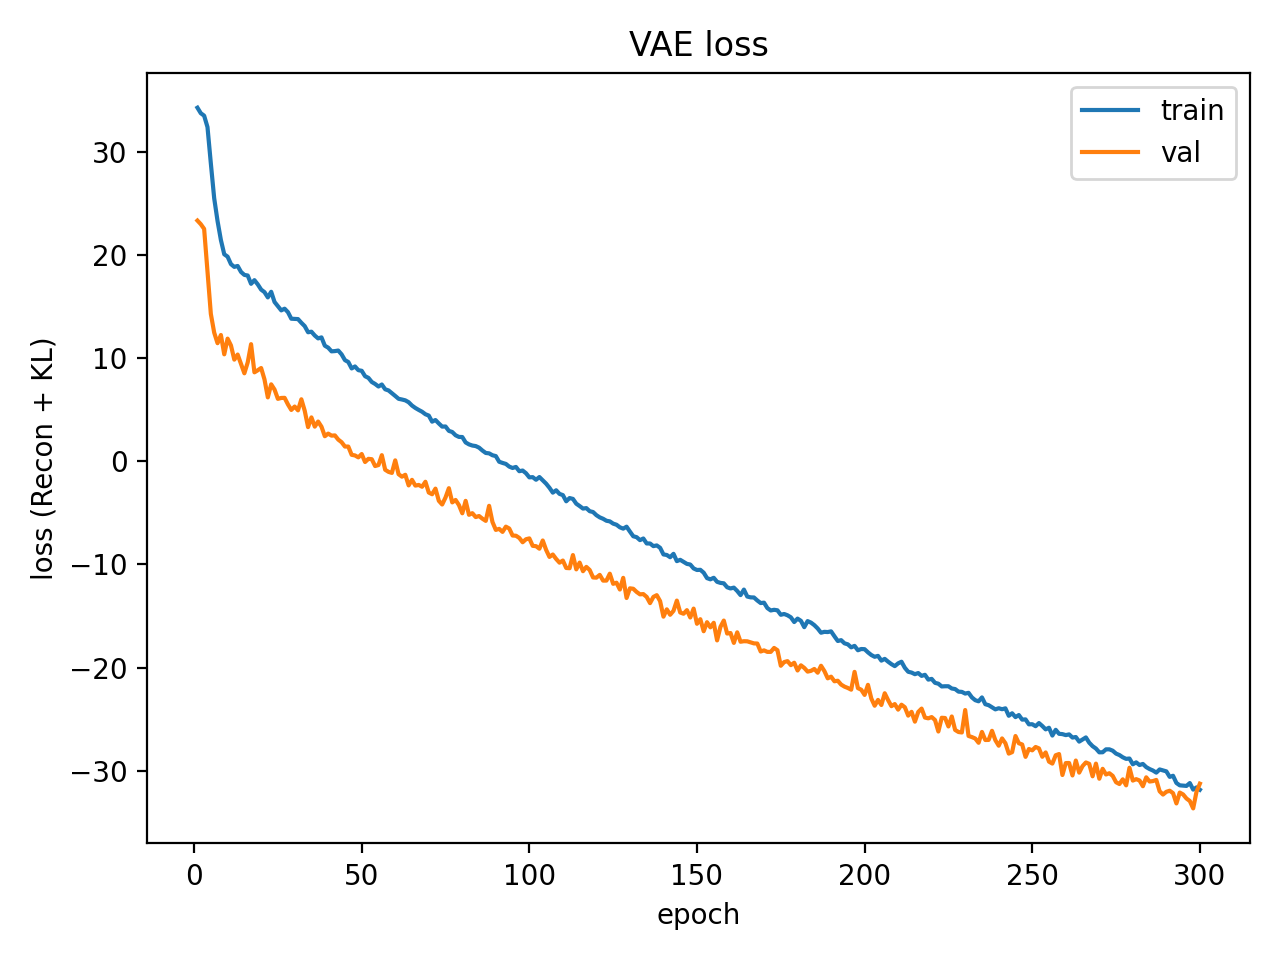
\includegraphics[width=\linewidth]{Figures/loss_curve.png}
    \caption{Training and validation loss for the VAE.}
    \label{fig:loss_curve}
\end{figure}

\subsection{Set-level identity coherence test}
To test whether identity is captured as a latent variable, we evaluate on a held-out test split containing six unseen proteins.
Rather than scoring individual conformers, we formulate a \emph{set-level} task.
For a set $S=\{y_i\}_{i=1}^K$, we compute a coherence score based on the encoder posterior means $\mu_\phi(y_i)$:
\begin{equation}
\mathrm{Score}(S) \;=\; - \frac{1}{K^2} \sum_{i,j} \|\mu_\phi(y_i)-\mu_\phi(y_j)\|^2.
\end{equation}
Intuitively, this measures how tightly a set clusters in latent space.

Positive sets consist of $K=5$ conformers drawn from the same test protein.
Negative sets are constructed by sampling one conformer from each of $K$ distinct test proteins, ensuring a strictly test-only evaluation.
We generate multiple sets per protein to reduce variance.

\subsection{Preliminary Results}
Despite the absence of identity supervision, the learned latent space exhibits significantly higher coherence for same-protein sets than for mixed sets.
Across 300 positive and 500 negative test-only sets, the coherence score achieves a ROC-AUC of \textbf{0.783}, indicating that same-identity sets are ranked as more coherent than mixed sets in \textbf{78\%} of random comparisons.
Mean coherence scores are $-7.00$ for same-identity sets versus $-10.52$ for mixed sets, indicating tighter latent clustering for conformational ensembles arising from a single protein.
These results demonstrate that protein identity, though not linearly apparent in raw mGLI features, is recoverable as a latent variable when multiple structural observations are considered jointly.


\section{Perspectives: Limitations and Future Directions}

To fairly interpret the results of this study, we highlight that we do not claim advantage over sequence alignment or residue-resolved contact maps when those signals are available, as identity inference in such settings is often trivial. The potential downstream application is inferring an underlying molecular identity from \emph{incomplete} structural data as often seen in experimental techniques like X-ray crystallography or Cryo-EM.

Methodologically, although ProteinConformers provides large ensembles that approximate continuous deformation landscapes, our study uses only a small number of conformers per protein, precluding faithful density estimation of conformational distributions.
In this regime, the VAE should be viewed primarily as a representation learner rather than a generative model of physical structure.

Future work may focus on training on larger subsets of ProteinConformers, leveraging the full range of continuous deformations. In such a setting, more expressive multimodal latent-variable models—such as mixture-based VAEs or normalizing flows—would be better suited to capture the inherently multi-modal structure of protein conformational landscapes and to support principled density-based inference.

\bibliographystyle{ACM-Reference-Format}
\bibliography{refs}

\appendix
\setcounter{figure}{0}
\renewcommand{\thefigure}{S\arabic{figure}}

\section{Interpreting the Protein-Centroid PCA Visualization}

Figure~\ref{fig:pca_centroids} visualizes a two-dimensional PCA projection of \emph{protein centroids}, where each centroid is computed as the mean mGLI embedding of all sampled conformers for a given protein.
This representation aggregates within-protein conformational variability into a single point per protein and provides a coarse summary of between-protein relationships in the original embedding space.

The centroids are broadly scattered without forming clearly separable clusters, and there is no obvious low-dimensional partition corresponding to protein identity, indicateing that even after averaging over conformers, identity information is not linearly separable in the raw mGLI feature space.
This motivates the probabilistic formulation adopted in the study:
protein identity is better modeled as a latent variable inferred from a distribution of observations, rather than as a property of any single structure or its mean representation.

\begin{figure}[H]
    \centering
    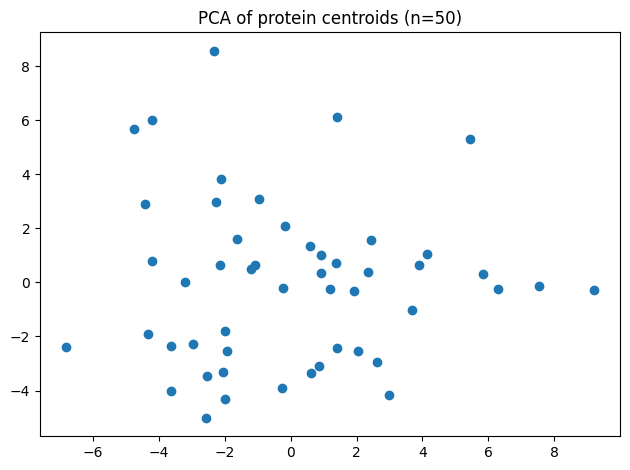
\includegraphics[width=\linewidth]{Figures/centroid_PCA.png}
    \caption{PCA projection of protein centroids, computed as the mean mGLI embedding over conformers for each protein.}
    \label{fig:pca_centroids}
\end{figure}

\end{document}